\section{Central Limit Theorem}
Recall that the Law of Last Numbers says that if $X_1, X_2, \dots$ are IID with finite means $\mu$ and variances $\sigma^2$, then the averages $A_n = \frac{1}{n} \sum_{i = 1}^{n} X_i \mapsto \mu$. In particular, we proved the LLN using Chebychev's Inequality, which gives 
\[\PR\left(|A_n - \mu| \geq C \frac{\sigma}{\sqrt{n}}\right) \leq \frac{1}{C^2}.\] 

The \textbf{Central Limit Theorem (CLT)} says more. The Central Limit Theorem says that the normalized averages \[Z_n = \frac{A_n - \mu}{\sigma / \sqrt{n}}\] \emph{converge in distribution} (this sequence of RV converges to another RV) to a standard Normal(0, 1) random variable $Z$. More precisely, this means that the CDFs \[F_{Z_n}(z) \mapsto F_{Z}(z)\] as $n \mapsto \infty$. 

\subsection{Relationship Between Chebychev's and CLT}
\begin{center}
    \begin{tabular}{||p{3in}|p{3in}||}
        \hline 
        \textbf{Chebyshev's Inequality} & \textbf{Central Limit Theorem} \\ 
        \hline \hline 
        \[\PR\left(|A_n - \mu| \geq C \frac{\sigma}{\sqrt{n}}\right) = \boxed{\PR(|Z_n| \geq C) \leq \frac{1}{C^2}}.\] 
        So, this gives us an upper-bound. Note that this works for \emph{any} $n$. 
        
        & 
        
        The CLT says that $\PR(|Z_n| \geq C) \mapsto \PR(|Z| \geq C)$, and 
        \[\PR(|Z| \geq C) = 2\int_{C}^{\infty} \frac{e^{-z^2 / 2}}{\sqrt{2\pi}} dz\]
        as $n \mapsto \infty$. Note that this works better for significantly large values of $n$.

        \bigskip 

        Note that \[\int_{C}^{\infty} \frac{e^{-z^2 / 2}}{\sqrt{2\pi}} dz\] is the area under the standard ``bell-shaped curve'' (i.e., the Normal(0, 1) PDF) to the right of $z = C$.
        \begin{center}
            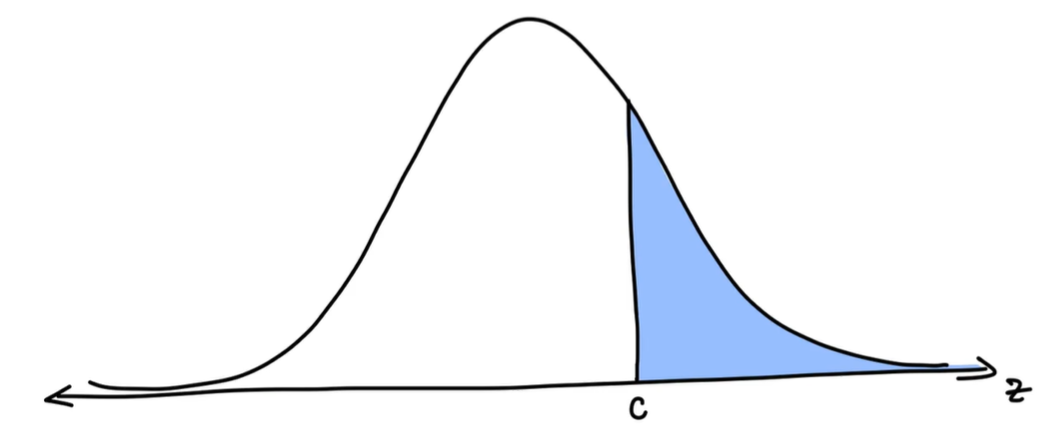
\includegraphics[scale=0.26]{assets/lec20clt.png}
        \end{center}
        As a remark, the integral above doesn't have an antiderivative, but we can make use of an online $z$-score calculator to find (very good approximations to) these values.
        \\ 
        \hline 
    \end{tabular}
\end{center}
\textbf{Remark:} For this class, we usually let $\mu = 0$, $\sigma = 1$, and $x$ be the value of interest ($|Z|$, for example).

\begin{mdframed}[nobreak=true]
    (Example.) We note that, by using a $z$-score calculator, we know that 
    \[\PR(|Z| \geq 2) = 2\PR(Z \geq 2) \approx 4.55\%.\]
    Using Chebyshev's Inequality, we find that the upperbound is $\leq \frac{1}{2^2} = 25\%$. 
\end{mdframed}

\begin{theorem}{Central Limit Theorem}{}
    Suppose that $X_1, X_2, \dots$ are IID with common mean $\mu < \infty$ and variance $\sigma^2 < \infty$. Put \[S_n = \sum_{i = 1}^{n} X_i.\] Then, for any $b \in \R$, 
    \[\PR\left(\frac{S_n - n \mu}{\sigma\sqrt{n}} \leq b\right) \mapsto \frac{1}{\sqrt{2\pi}} \int_{-\infty}^{b} e^{-z^2 / 2}dz.\]
    Note that $\mathbb{E}(S_n) = n\mu$ and $SD(S_n) = \sqrt{\text{Var}(S_n)} = \sigma\sqrt{n}.$
\end{theorem}
\textbf{Remarks:} 
\begin{itemize}
    \item Note that 
    \[\frac{S_n - n\mu}{\sigma\sqrt{n}} = \frac{A_n - \mu}{\sigma / \sqrt{n}}\]
    where $S_n = \sum_{i = 1}^{n} X_i$ is the sum and $A_n = \frac{1}{n}S_n = \frac{1}{n} \sum_{i = 1}^{n} X_i$ is the average.  

    \item The key is that you do not need to know the actual distribution of the $X_i$'s. We only need to know that they are IIDs (and that their means are variances exist). So, in essense, \emph{the CLT gives useful information about averages of a distribution without needing to know what the distribution really is.}
\end{itemize}

Note that, when applying the CLT to \emph{discrete} IID sequences $X_1, X_2, \dots$, it is often useful to make a ``discrete adjustment'' to get a slightly better approximation. 

\begin{mdframed}[]
    (Example: Normal Approximation to the Binomial.) Recall that a Binomial($n, p$) RV $X_n$ is the sum of $n$ IID Bernoulli($p$) RVs, and that its mean is $np$ and variance $npq$, where $q = 1 - p$. Thus, by the CLT, 
    \[\PR(i \leq X_n \leq j) \approx \PR\left(\frac{i - np}{\sqrt{npq}} \leq Z \leq \frac{j - np}{\sqrt{npq}}\right)\]
    for large $n$.

    \bigskip 

    We can, however, get a better approximation (unless $n$ is very large, in which case it makes little difference) if we instead approximate
    \[\PR(i \leq X_n \leq j) \approx \PR\left(\frac{i - 1/2 - np}{\sqrt{npq}} \leq Z \leq \frac{j + 1/2 - np}{\sqrt{npq}}\right).\]
    The reason why is because this makes a correction to get all of the relevant ``bars.''
\end{mdframed}

\begin{mdframed}[]
    (Example.) A fair coin is tossed 100 times. Estimate the probability that ``Heads'' is tossed between 40 and 60 times. 

    \bigskip 

    Let $S_n = \sum_{i = 1}^{n} X_i$ where $X_i$ indicates if the $i$th toss is ``Heads.'' Letting $X_i$ be a Bernoulli, where $X_i$ is 1 if the $i$th toss is ``Heads'' and 0 otherwise. Then, applying the Binomial approximation, we have  
    \begin{equation*}
        \begin{aligned}
            \PR(40 \leq S_n \leq 60) &= \PR\left(\frac{40 - 0.5 - 100(0.5)}{\sqrt{100(0.5)(1 - 0.5)}} \leq Z \leq \frac{60 + 0.5 - 100(0.5)}{\sqrt{100(0.5)(1 - 0.5)}}\right) \\ 
                &= \PR(|Z| \leq 2.1).
        \end{aligned}
    \end{equation*}
    So, using the online calculator, we want to compute 
    \[\PR(-2.1 \leq Z \leq 2.1).\]
    Doing this (letting $\mu = 0$, $\sigma = 1$, $x = 2.1$, and $\PR(-|x| < X < |x|)$ in the dropdown menu) gives us 96.42\%.

    \bigskip 

    Without the discrete correction, we would have found 
    \[\PR(-2 \leq Z \leq 2) \approx 95.45\%.\]
    But, by calculating the true probability, we get 
    \[\frac{1}{2^{100}} \sum_{i = 40}^{60} \binom{100}{i} = 96.479\dots\%.\]
\end{mdframed}


\subsection{Applications}
Recall that you do not need to know the distributions of the $X_i$. You also -- in many cases -- do not need a very large sample size to obtain fairly accurate results. This is because, for many distributions (as long as the unknown distribution is not highly asymmetric or unusual), convergence to the Normal is often reasonably fast. So, generally speaking, $n \geq 30$ is a good sample size. 

\subsubsection{z-Distribution}
\begin{mdframed}[]
    (Example.) In his 2020 interview with PBS NewsHour about his work on post-election auditing, the UC Berkeley statistician Professor Philip Stark gave the analogy of cooking a pot of soup. 

    \bigskip 

    In order to know if it is tasty/too salty/etc., you do not need to drink the whole pot of soup. Instead, as long as you mix up the pot sufficiently well, even just one spoonful is enough, no matter how large the pot is. 
\end{mdframed}

\begin{mdframed}[]
    (Example.) A surveyor wants to measure the distance $d$ between two locations $A$ and $B$. She knows there will be some degree of error (due to human error, atmospheric distortions, etc.) Therefore, instead of taking just one reading, she decides to take $n = 36$ of them. Assuming the measurements are IID, and that the SD associated with measurements is $\sigma = 0.001$ (perhaps based on past experience), what can we say about the true distance $d$? 

    \bigskip 

    It is natural to expect that the expected value of any given reading is $\mu = d$ (at least, we would hope so). Of course, this is just an expectation. Now, if $X_1, X_2, \dots$ are an IID sequence of measurements, then 
    \[\frac{1}{n} \sum_{i = 1}^{n} X_i \mapsto d\]
    as $n \mapsto \infty$. But, for just $n = 36$ measurements, what can we say about $d$? Can we at least estimate $d$ within some reasonable degree of freedom? 

    \bigskip 

    Now, note that by CLT, \[\frac{A_n - d}{\sigma / \sqrt{n}}\] is asymptotically Normal(0, 1), where recall \[A_n = \frac{1}{n}\sum_{i = 1}^{n} X_i\] is the sample average. 

    \bigskip 

    Now, if $Z$ is Normal(0, 1), then $\PR(|Z| \leq 1.96) \approx 95\%$ (here, we just arbitrarily picked 95\% and then found 1.96 through an online calculator). Therefore, 
    \[\PR\left(\left|\frac{A_n - d}{\sigma / \sqrt{n}}\right| \leq 1.96\right) \approx 95\%.\]
    This is useful because everything here is known (we know the standard deviation, sample average, and $n$) \emph{except} for the true distance $d$. Now, note that 
    \[\left|\frac{A_n - d}{\sigma / \sqrt{n}}\right| = \left|\frac{A_n - d}{0.001 / \sqrt{36}}\right| \leq 1.96\] 
    if $d \in \left[A_n \pm 1.96 \frac{0.001}{6}\right] = [A_n \pm 0.000327]$. This is known as a \textbf{confidence interval}. 

    \bigskip 

    Now, suppose that the sample average after 36 readings is 1.0045. Then, we would say that we are ``95\% confident'' that the true distance $d$ is somewhere in the interval $[1.0045 \pm 0.000327] = [1.004173, 1.004827]$. This is what is called a \textbf{95\% confidence interval (CI)}.
\end{mdframed}
\textbf{Remarks:}
\begin{itemize}
    \item Note that the sample average is denoted by $\overline{\mu}$, $\hat{\mu}$, $\overline{x}$, etc.
    \item Note that $[a \pm b] = [a - b, a + b]$. 
\end{itemize}

More generally, to make a $(100)(1 - \alpha)\%$ CI for an unknown mean $\mu$, supposing the true standard deviation $\sigma$ is known, we 
\begin{enumerate}[(a)]
    \item Find $z_*$ such that $\PR(|Z| \leq z_*) = 100(1 - \alpha)\%$. Note that, for $\alpha = 0.1, 0.05, 0.01$ (corresponding to $90, 95, 99\%$ confidence), we have $z_* \approx 1.64, 1.96, 2.58$. As $\alpha$ decreases, naturally $z_*$ (and hence the width of the CI) decreases. 
    \item Find the sample average $\hat{\mu}$. 
    \item Then, we can construct the confidence interval 
    \[\left[\hat{\mu} \pm z_* \frac{\sigma}{\sqrt{n}}\right].\]
    Notice that there is a tradeoff:
    \begin{itemize}
        \item The width of the interval will increase as the confidence level increases. 
        \item As we increase the size of the sample, the width of the confidence interval will decrease.  
    \end{itemize}
\end{enumerate}
Interpretating what, for example, ``95\% confident'' means here is theoretically subtle. For instance, notice that 
\[\PR\left(\mu \in \left[\hat{\mu} \pm z_* \frac{\sigma}{\sqrt{n}}\right]\right) = 95\%\]
is non-sensical. Just because we do not know $\mu$ dies not make it random; it either is in the CI or it isn't. Therefore, this probability is in fact either 0 or 1, but we do not know which. 

\bigskip 

Note that the confidence interval is random, not $\mu$. This is because we took a random sample. Interpreting what ``95\% confident'' means actually involves another application of the CLT. 

\bigskip 

Specifically, what we mean here is that if we were to build a large number of IID CIs, in exactly the same way that we did this \emph{one} CI, then 
\begin{itemize}
    \item provided that $n$ is reasonably large, about 95\% of them would contain the true value of $\mu$,
    \item and, in this sense, we are ``95\% confident'' that this \emph{one} CI we have made contains the true value of $\mu$. 
\end{itemize}

\subsubsection{t-Distribution}
More often in practice, both $\mu$ and $\sigma$ are unknown. In this case, experience has shown that instead of using the Normal distribution, it is better to use an alternative -- but related -- distribution called \textbf{Student's $t$-distribution.} This makes the most difference when the sample size $n$ is small. In fact, as $n \mapsto \infty$, the student's $t$-distribution converges to the standard Normal. So, if $n$ is large, the improvement is negligible. 

\bigskip 

If the true standard deviation $\sigma$ is unknown, then we must estimate it using the sample standard deviation. 
\[\hat{\sigma} = \sqrt{\frac{1}{n - 1} \sum_{i = 1}^{n} (X_i - \hat{\mu})^2}.\]
The reason we use $n - 1$ instead of $n$ is to further account for the imprecision in our estimates. statisticians say that 1 ``degree of freedom'' has already been lost, since we had to first estimate $\mu$, before we have estimated $\sigma$. 

\bigskip 

Therefore, when the true mean $\mu$ and standard deviation are both unknown, we construct a $(100)(1 - \alpha)\%$ CI using the formula 
\[\left[\hat{\mu} \pm t_* \frac{\hat{\sigma}}{\sqrt{n}} \right]\]
instead of 
\[\left[\hat{\mu} \pm z_* \frac{\sigma}{\sqrt{n}}\right]\]
as before. The two differences between these two formulas are 
\begin{itemize}
    \item We replaced $\sigma$ with the estimate $\hat{\sigma}$ (since $\sigma$ is unknown).
    \item We are using a $t$-score instead of a $z$-score.
\end{itemize}
Here, $t_*$ is the value for which $\PR(|T| \leq t_*) = 1 - \alpha$, where $T$ has Student's $t$-distribution with $n - 1$ degrees of freedom. Here, we can use an online calculator (note that $v = n - 1$ in the calculator).

\bigskip 

We can then use these ideas to run statistical hypothesis tests.

\begin{mdframed}[]
    (Example.) Suppose that we would like to determine if the usual body temperature of humans differs from 98.6 degrees F. Note that we do not know the true mean $\mu$ nor the true standard deviation $\sigma$. 

    \bigskip 

    Suppose we take a random sample of 130 temperatures (so we know all of the $X_i$'s), and find that $\hat{\mu} = 98.25$ and $\hat{\sigma} = 0.73$. At the 0.05 (5\%) ``significance level,'' can we reject the \textbf{null hypothesis} that $\mu = 98.6$. This means that if we reject the hypothesis, then there's only a 5\% chance we're making a mistake by doing so. In other words, if we reject the hypothesis that $\mu = 98.6$, then we can do so with the probability of 5\% that we're making a mistake.
    
    \bigskip 

    Under the null hypothesis, the statistic 
    \[T = \frac{\hat{\mu} - 98.6}{\sigma^2 / \sqrt{n}}\]
    is approximately a Student's $t$ with $n - 1 = 129$ degrees of freedom. Therefore, $\PR(|T| \geq 1.978) = 5\%$. There's only a 5\% chance that we will observe something as extreme at something like 1.978. So, that means that if we get a statistics that's larger than 1.978, then that means that there's only a 5\% chance that it's really true that 98.6 is the true temperature. 

    \bigskip 

    Now, let's suppose that $\hat{\mu} = 98.25$ and $\hat{\sigma} = 0.73$ and so 
    \[T = \frac{98.25 - 98.6}{0.73 / \sqrt{130}} \approx -5.47,\]
    which is a lot more extreme (and so even more unlikely) than 1.978. Hence, under the null hypothesis, the chance of us observing this statistic $T \approx -5.47$ is (much) less than 5\%. Therefore, at the $\alpha = 0.05$ significance level, we reject the null hypothesis, in favor of the \textbf{alternative hypothesis} that the true average temperature is lower than 98.6 degrees F. 
\end{mdframed}